\chapter{التآكل والحماية}\label{ch:b2:corrosion}

اترك قطرة من الماء المالح على قطعة نظيفة من الفولاذ. بعد يوم يكون الفلز
منقورًا في مركز القطرة، بينما يتكوّن الصدأ حلقةً قرب
حافتها، حيث يذوب أكسجين الهواء. فالحديد يذوب حيث يكون
الأكسجين أقل، ويُختزل الأكسجين حيث يكون أكثر: فالقطرة
خلية لم يبنها أحد، مقصورة الدارة عبر الفلز نفسه. يقرأ هذا
الفصل التآكل على منحنيات شدة التيار--الجهد، ويفسر لماذا لا تصدأ
صفيحة مجلفنة مخدوشة بينما تصدأ علبة مقصدرة مخدوشة، ويصمم
حماية خط أنابيب مدفون.

\begin{recall}
مجلد السنة الأولى: مخططات الجهد--pH للفلزات ومناطق المناعة والتآكل
\omterm{def:b2:corrosion:passivation}{والتخميل} فيها («وكون الطبقة واقيةً مسألة حركية»).
\Cref{ch:b2:current-potential-curves}: منحنيات شدة التيار--الجهد، والتيارات
الحدية. \Cref{ch:b2:batteries-electrolysis}: \omterm{def:b2:batteries-electrolysis:mixed-potential}{الجهد المختلط}. والمجلد
المدرسي: التآكل، والصدأ، والجلفنة.
\end{recall}

\begin{omfigure}
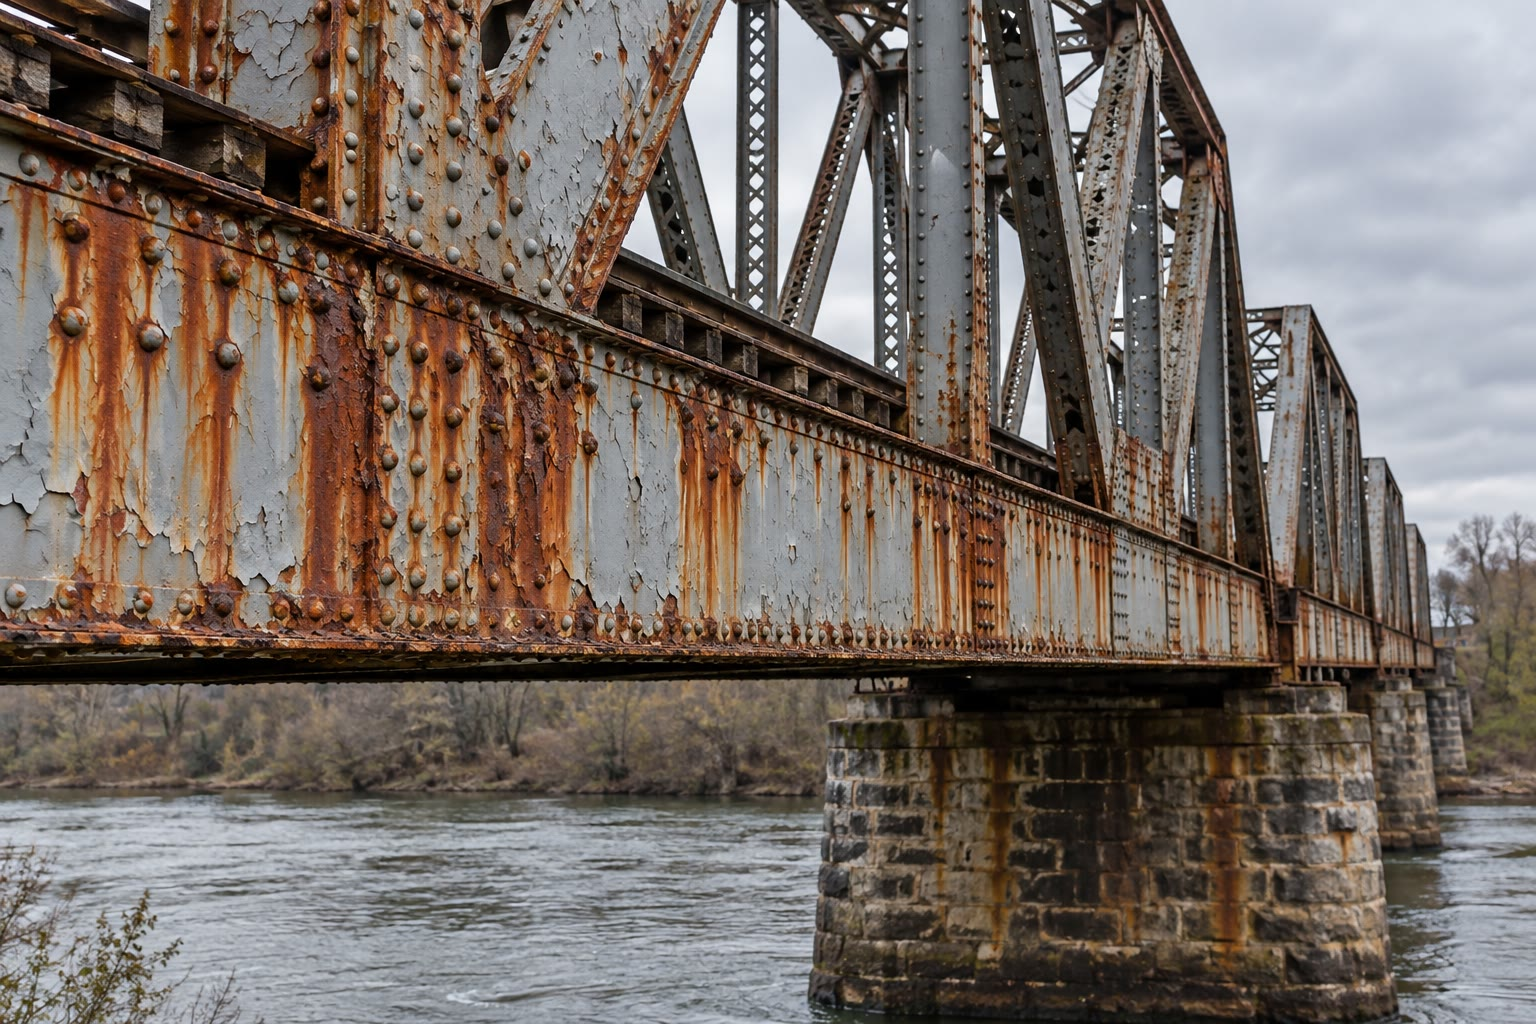
\includegraphics[width=0.62\linewidth]{images/book3/ai/b2-12-rusty-bridge.jpg}

{\small جسر سكة حديدية قديم مبرشم. تسيل خطوط الصدأ من المسامير
والوصلات، حيث يبقى الماء والأكسجين أطول مدة ويتلف الطلاء
أولًا.}
\end{omfigure}

\section{التآكل الرطب خليةً مقصورة الدارة}

في ماء يحوي أكسجينًا مذابًا يتأكسد الحديد، \ce{Fe -> Fe^2+ + 2e-}،
وتؤخذ الإلكترونات على قطعة الفلز نفسها باختزال
ثنائي الأكسجين، \ce{O2 + 2H2O + 4e- -> 4OH-} (وفي الوسط الحمضي أيضًا بالتفاعل \ce{2H+ + 2e- -> H2}). وتلتقي
أيونات الحديد(II) وأيونات الهيدروكسيد في الماء، ويحوّل تأكسد إضافي بالهواء
راسبها إلى صدأ، وهو أكسيد حديد(III) مميَّه.

\begin{definition}[التآكل المنتظم]\label{def:b2:corrosion:uniform}
\emph{التآكل المنتظم}\index{تآكل منتظم} تآكل فلز تجري أكسدته
واختزال المؤكسد فيه عند مواقع موزعة بانتظام
على سطحه. و\emph{جهد التآكل}\index{جهد التآكل}
هو \omterm{def:b2:batteries-electrolysis:mixed-potential}{الجهد المختلط} الذي يأخذه الفلز عندئذ، و\emph{تيار
التآكل}\index{تيار التآكل} هو \omterm{def:b2:current-potential-curves:ie-curve}{التيار المصعدي} لأكسدة
الفلز عند ذلك الجهد.
\end{definition}

\begin{omfigure}
\begin{tikzpicture}
\begin{axis}[omie, width=0.82\linewidth, height=5.6cm, xmin=-1.1, xmax=0.5,
  ymin=-1.6, ymax=1.6, xlabel={$E$}, ylabel={$i$}, clip=true, clip mode=individual,
  axis y line=left]
\addplot[omanodic] table[x=E, y=i] {figdata/out/bachelor-2-ie-curves-i-Fe.dat};
\addplot[omcathodic] table[x=E, y=i] {figdata/out/bachelor-2-ie-curves-i-O2.dat};
\addplot[omcathodic, densely dashed] table[x=E, y=i, y expr=-\thisrow{i}] {figdata/out/bachelor-2-ie-curves-i-O2.dat};
\draw[densely dotted] (axis cs:-0.394,-1.0) -- (axis cs:-0.394,1.0);
\fill (axis cs:-0.394,1.0) circle (1.4pt);
\node[font=\scriptsize, anchor=south east] at (axis cs:-0.40,1.02) {$i_{\text{تآكل}}$};
\node[font=\scriptsize, anchor=north west] at (axis cs:-0.39,-0.03) {$E_{\text{تآكل}}$};
\node[font=\scriptsize, omThm, anchor=west] at (axis cs:-0.35,1.4) {\babelsublr{\ce{Fe} $\to$ \ce{Fe^2+}}};
\node[font=\scriptsize, omDef, anchor=north west] at (axis cs:-0.75,-1.05) {\foreignlanguage{arabic}{\babelsublr{\ce{O2} $\to$ \ce{OH-}}، استواء الانتشار}};
\end{axis}
\end{tikzpicture}

{\small مخطط إيفانز للحديد في ماء متعادل مهوّى (منحنيات نموذجية). ويُرسم
المنحنى المهبطي لثنائي الأكسجين أيضًا معكوسًا نحو الأعلى (متقطعًا): \omterm{def:b2:corrosion:uniform}{فجهد
التآكل} هو حيث يلاقي المنحنى المصعدي للحديد. ولأن
اختزال ثنائي الأكسجين قد بلغ هناك استواء انتشاره، يساوي \omterm{def:b2:corrosion:uniform}{تيار التآكل}
\omterm{def:b2:current-potential-curves:limiting-current}{التيار الحدي} للأكسجين: فتحريك الماء أو تهويته
يجعل الحديد يتآكل أسرع.}
\end{omfigure}

\begin{proposition}[سرعة التآكل]\label{prop:b2:corrosion:rate}
الفلز ذو الكتلة المولية $M$ والكثافة $\rho$، المتأكسد مع $n$ إلكترونًا لكل
ذرة تحت كثافة تيار تآكل $j_{\text{تآكل}}$ (التيار لكل وحدة مساحة)،
يفقد لكل وحدة مساحة ووحدة زمن الكتلة $j_{\text{تآكل}}M/(nF)$، أي
سمكًا
\[
  \frac{de}{dt} = \frac{j_{\text{تآكل}}\,M}{nF\rho} .
\]
\end{proposition}

\begin{proof}
حسب \cref{prop:b2:current-potential-curves:current-rate}، تؤكسد كثافة \omterm{def:b2:current-potential-curves:ie-curve}{التيار
المصعدي} $j_{\text{تآكل}}$ مقدار $j_{\text{تآكل}}/(nF)$ مولًا من الفلز لكل وحدة مساحة ووحدة
زمن؛ نضرب في $M$ للحصول على الكتلة ونقسم على $\rho$ للحصول على السمك.
\end{proof}

\begin{example}[الحديد عند \qty{10}{\micro A/cm^2}]\label{ex:b2:corrosion:rate}
مع $j = \qty{0.10}{A/m^2}$، و$M = \qty{55.845}{g/mol}$، و$n = 2$، و$\rho =
\qty{7.87}{g/cm^3}$: $de/dt = 0.10 \times 55.845/(2 \times 96\,485 \times 7.87
\times 10^6) = \qty{3.7e-12}{m/s}$، أي \qty{0.12}{mm} في السنة.
% ledger: aw:Fe, rho:Fe, const:F
\end{example}

\section{التآكل التفاضلي}

\begin{definition}[التآكل التفاضلي]\label{def:b2:corrosion:differential}
\emph{التآكل التفاضلي}\index{تآكل تفاضلي} تآكل تنفصل فيه
المواقع المصعدية عن المهبطية، فيتأكسد الفلز
بالأفضلية عند المواقع المصعدية. ويكون \emph{تآكلًا
غلفانيًا}\index{تآكل غلفاني} حين يشترك فلزان مختلفان في تماس
كهربائي في الإلكتروليت نفسه، و\emph{تهوية
تفاضلية}\index{تهوية تفاضلية} حين يتعرض فلز واحد لمياه
مختلفة المحتوى من الأكسجين.
\end{definition}

\begin{proposition}[فلزان متلامسان]\label{prop:b2:corrosion:galvanic}
حين يُغمر فلزان في تماس كهربائي في الماء المهوّى نفسه، يأخذان
جهدًا مختلطًا واحدًا. والفلز الذي جهد تآكله أدنى
يصير المصعد ويتآكل أسرع منه وحده؛ ويصير الآخر مهبطًا،
يُختزل عليه ثنائي الأكسجين، فيُحمى.
\end{proposition}

\begin{proof}
الفلزان الموصولان بموصل ذي مقاومة مهملة يكونان عند الجهد
نفسه، حيث يساوي مجموع كل التيارات المصعدية سالب مجموع كل
التيارات المهبطية. والمنحنى المصعدي للفلز الأقل نبلًا يصعد أولًا؛
فيحمل عند الجهد المشترك كل \omterm{def:b2:current-potential-curves:ie-curve}{التيار المصعدي} تقريبًا، ويُختزل
الأكسجين على السطح المبلل كله، بما فيه الفلز الأنبل،
الذي يكون تياره المصعدي الخاص مهملًا هناك.
\end{proof}

\begin{omfigure}
\begin{tikzpicture}
\begin{axis}[omie, width=0.82\linewidth, height=5.6cm, xmin=-1.1, xmax=0.5,
  ymin=-2.4, ymax=2.4, xlabel={$E$}, ylabel={$i$}, clip=true, clip mode=individual,
  axis y line=left]
\addplot[omanodic] table[x=E, y=i] {figdata/out/bachelor-2-ie-curves-i-Fe.dat};
\addplot[omanodic, densely dashed] table[x=E, y=i] {figdata/out/bachelor-2-ie-curves-j-Zn.dat};
\addplot[omcathodic] table[x=E, y=i] {figdata/out/bachelor-2-ie-curves-i-O2.dat};
\addplot[omcathodic, densely dashed] table[x=E, y=i] {figdata/out/bachelor-2-ie-curves-j-O2Cu.dat};
\fill (axis cs:-0.394,1.0) circle (1.4pt);
\fill (axis cs:-0.794,1.0) circle (1.4pt);
\fill (axis cs:-0.366,2.0) circle (1.4pt);
\draw[densely dotted] (axis cs:-1.1,1.0) -- (axis cs:-0.394,1.0);
\draw[densely dotted] (axis cs:-1.1,2.0) -- (axis cs:-0.366,2.0);
\node[font=\scriptsize, anchor=south west] at (axis cs:-0.38,0.95) {الحديد وحده};
\node[font=\scriptsize, anchor=west] at (axis cs:-0.35,2.0) {حديد + نحاس};
\node[font=\scriptsize, anchor=south east] at (axis cs:-0.80,1.05) {حديد + زنك};
\node[font=\scriptsize, omThm, anchor=north west] at (axis cs:-0.98,0.75) {زنك};
\node[font=\scriptsize, omThm, anchor=north west] at (axis cs:-0.55,0.75) {حديد};
\node[font=\scriptsize, omDef, anchor=north east] at (axis cs:0.45,-2.05) {\foreignlanguage{arabic}{\ce{O2} على حديد + نحاس}};
\node[font=\scriptsize, omDef, anchor=north east] at (axis cs:0.45,-1.05) {\foreignlanguage{arabic}{\ce{O2} على الحديد}};
\end{axis}
\end{tikzpicture}

{\small الحديد موصولًا بفلزات أخرى (منحنيات نموذجية). مع الزنك، ينخفض الجهد
المشترك إلى حيث يحمل الزنك \omterm{def:b2:current-potential-curves:ie-curve}{التيار المصعدي}: فيُحمى الحديد، ويتآكل
الزنك. ومع النحاس، تتضاعف المساحة المهبطية المتاحة للأكسجين: فيتضاعف
تيار تآكل الحديد أيضًا.}
\end{omfigure}

\begin{proposition}[التهوية التفاضلية]\label{prop:b2:corrosion:aeration}
على فلز معرَّض لمياه مختلفة المحتوى من الأكسجين، تكون المنطقة الأقل تهوية
مصعدية فتتآكل؛ والمنطقة الأفضل تهوية مهبطية.
\end{proposition}

\begin{proof}
حيث يكون محتوى الأكسجين أعلى يكون للمزدوجة $\ce{O2}/\ce{OH-}$ جهد نرنست
أعلى \omterm{def:b2:current-potential-curves:limiting-current}{وتيار حدي} أكبر: فيقع المنحنى المهبطي أعلى
ويمتد أبعد. والفلز، وهو موصل واحد، يستقر عند جهد واحد؛
ويجب موازنة \omterm{def:b2:current-potential-curves:ie-curve}{التيار المهبطي} الكبير المتاح في المنطقة المهواة \omterm{def:b2:current-potential-curves:ie-curve}{بتيار
مصعدي}، يجري حيث يمكن أكسدة الفلز مع قليل من
منافسة اختزال الأكسجين، أي في المنطقة الضعيفة التهوية. فتتركز
الأكسدة هناك.
\end{proof}

\begin{omfigure}
\begin{tikzpicture}[font=\small, >={Stealth}]
  \fill[black!20] (-4.2,-0.7) rectangle (4.2,0);
  \node[font=\scriptsize] at (3.7,-0.35) {فولاذ};
  \fill[omDef!15] (-3.4,0) .. controls (-2.9,2.2) and (2.9,2.2) .. (3.4,0) -- cycle;
  \draw[thick, omDef] (-3.4,0) .. controls (-2.9,2.2) and (2.9,2.2) .. (3.4,0);
  \fill[omProp!80] (-0.7,0) arc[start angle=180, end angle=360, x radius=0.7, y radius=0.22] -- cycle;
  \fill[brown!70!black] (-1.9,0.12) ellipse (0.45 and 0.11);
  \fill[brown!70!black] (1.9,0.12) ellipse (0.45 and 0.11);
  \node[font=\scriptsize, align=center] at (0,2.45) {\foreignlanguage{arabic}{\ce{O2} من الهواء}};
  \draw[->, thick, omDef] (-1.0,2.25) -- (-2.6,0.35);
  \draw[->, thick, omDef] (1.0,2.25) -- (2.6,0.35);
  \node[font=\scriptsize, align=center, anchor=east] at (-4.1,1.3) {\shortstack{\foreignlanguage{arabic}{مهبط}\\\foreignlanguage{arabic}{(الحافة)}}};
  \draw[->, thin] (-4.1,1.3) -- (-3.05,0.12);
  \node[font=\scriptsize, align=center, anchor=west] at (4.1,1.3) {حلقة الصدأ};
  \draw[->, thin] (4.1,1.3) -- (2.3,0.2);
  \draw[->, omThm] (-0.4,-0.3) .. controls (-1.2,-0.5) and (-2.4,-0.5) .. (-3.0,-0.15);
  \draw[->, omThm] (0.4,-0.3) .. controls (1.2,-0.5) and (2.4,-0.5) .. (3.0,-0.15);
  \draw[->, thin] (0,-1.05) -- (0,-0.25);
  \node[font=\scriptsize, anchor=north] at (0,-1.05) {\shortstack{\foreignlanguage{arabic}{مصعد (المركز): \ce{Fe -> Fe^2+ + 2e-}}}};
  \node[font=\scriptsize, omThm, anchor=north] at (0,-1.45) {تجري الإلكترونات عبر الفولاذ إلى الحافة};
  \node[font=\scriptsize, anchor=north] at (0,-1.85) {\shortstack{\foreignlanguage{arabic}{مهبط (الحافة): \ce{O2 + 2H2O + 4e- -> 4OH-}}}};
\end{tikzpicture}

{\small قطرة إيفانز على الفولاذ، رسم تخطيطي. يذوب الأكسجين عند السطح
ويبلغ الفلز في الغالب قرب الحافة الرقيقة للقطرة، التي تصير
المهبط؛ أما المركز، المحروم من الأكسجين، فهو المصعد ويُنقر. وتلتقي
أيونات الحديد(II) وأيونات الهيدروكسيد بينهما، حيث يترسب الصدأ
على هيئة حلقة.}
\end{omfigure}

تهاجم الآلية نفسها الشقوق، وأجزاء المنشأة الواقعة تحت راسب
أو حشية، والركيزة الفولاذية في البحر تحت خط الماء بقليل، حيث
يكون الماء أقل تهوية منه عند السطح.

\begin{method}[تشخيص تآكل]\label{met:b2:corrosion:diagnose}
\begin{enumerate}
  \item اذكر الفلزات المتلامسة والإلكتروليت؛ وتحقق من أنها
        موصولة كهربائيًا.
  \item في حالة فلزين، يكون المصعد هو الفلز ذو \omterm{def:b2:corrosion:uniform}{جهد التآكل} الأدنى (وهو عادة
        ذو الجهد المعياري الأدنى).
  \item في حالة فلز واحد، جِد المناطق الأقل تهوية (الشقوق، وما تحت الرواسب،
        وقاع القطرة): فهي مصعدية.
  \item يحدد السرعةَ التفاعلُ المهبطي (إمداد الأكسجين، ومساحة المهبط):
        فالمصعد الصغير على مهبط كبير يتآكل بسرعة.
\end{enumerate}
\end{method}

\section{التخميل}

\begin{definition}[التخميل]\label{def:b2:corrosion:passivation}
\emph{التخميل}\index{تخميل} هو الانخفاض الشديد لسرعة تآكل
فلز حين تغطيه طبقة رقيقة متراصة ملتصقة من
أكسيده، هي \emph{الغشاء المخمِّل}\index{غشاء مخمِّل}، تفصله عن
المحلول. ويُقال عن الفلز في هذه الحالة إنه مخمَّل.
\end{definition}

\begin{proposition}[استواء التخميل]\label{prop:b2:corrosion:passivity}
يصعد المنحنى المصعدي لفلز قابل \omterm{def:b2:corrosion:passivation}{للتخميل} من جهد تآكله،
ويبلغ قمة، ثم ينخفض إلى تيار \omterm{def:b2:corrosion:passivation}{تخميل} صغير شبه ثابت على
مجال من الجهود، قبل أن يصعد من جديد عند الجهود العالية (منطقة ما بعد
\omterm{def:b2:corrosion:passivation}{التخميل}: أكسدة الغشاء أو الماء). ويمكن أن تنهار حالة \omterm{def:b2:corrosion:passivation}{التخميل}
موضعيًا، مثلًا تحت تأثير أيونات الكلوريد، معطيةً نُقَرًا.
\end{proposition}

\begin{proof}[تعليل]
عند \omterm{def:b2:current-potential-curves:overpotential}{فرط الجهد} الصغير يذوب الفلز العاري أسرع فأسرع. وبعد
عتبة يصير الأكسيد مستقرًا عند السطح (منطقة \omterm{def:b2:corrosion:passivation}{التخميل} في
مخطط الجهد--pH) ويكوّن غشاءً لا تتحرك الأيونات عبره إلا ببطء: فينهار
التيار إلى هذا التدفق الصغير. وعند الجهود العالية يتأكسد الغشاء نفسه
إلى أنواع ذائبة، أو يتأكسد الماء عليه. وأيونات الكلوريد، الصغيرة
والقوية التعقيد، تستطيع إذابة الغشاء عند نقاط ضعفه، حيث يتآكل الفلز
العاري عندئذ مصعدًا صغيرًا أمام مهبط مخمَّل ضخم. وشكل
المنحنى هنا نموذج.
\end{proof}

\begin{omfigure}
\begin{tikzpicture}
\begin{axis}[omie, width=0.82\linewidth, height=5.4cm, xmin=-0.7, xmax=1.5,
  ymin=-0.1, ymax=1.3, xlabel={$E$}, ylabel={$i$}, clip=true, clip mode=individual,
  axis y line=left]
\addplot[omanodic] table[x=E, y=i] {figdata/out/bachelor-2-ie-curves-k.dat};
\node[font=\scriptsize, anchor=south] at (axis cs:-0.33,1.0) {نشط};
\node[font=\scriptsize, anchor=south] at (axis cs:0.5,0.06) {استواء التخميل};
\node[font=\scriptsize, anchor=east] at (axis cs:1.25,0.9) {ما بعد التخميل};
\draw[<-, thin] (axis cs:-0.2,0.55) -- (axis cs:0.15,0.7) node[right, font=\scriptsize] {يتكوّن الغشاء};
\end{axis}
\end{tikzpicture}

{\small المنحنى المصعدي لفلز قابل \omterm{def:b2:corrosion:passivation}{للتخميل} (نموذج). التيار، الكبير ما دام
الفلز العاري يذوب، ينهار حين يتكوّن \omterm{def:b2:corrosion:passivation}{الغشاء المخمِّل}، ويبقى
صغيرًا على مجال واسع من الجهود قبل الصعود الذي يلي منطقة ما بعد \omterm{def:b2:corrosion:passivation}{التخميل}.}
\end{omfigure}

تحوي أنواع الفولاذ المقاوم للصدأ ما يكفي من الكروم لتكوين \omterm{def:b2:corrosion:passivation}{غشاء مخمِّل} من أكسيد الكروم
يرمم نفسه في الهواء؛ ويحمي الألومنيوم غشاءُ الألومينا، وهو ما
يجعل فلزًا يقع بعيدًا تحت الهيدروجين في السلسلة صالحًا لإطارات النوافذ
وعلب المشروبات. ويخضر النحاس في الهواء الطلق، والزنجار طبقة من
أملاح النحاس القاعدية تبطئ الهجوم اللاحق.

\begin{omfigure}
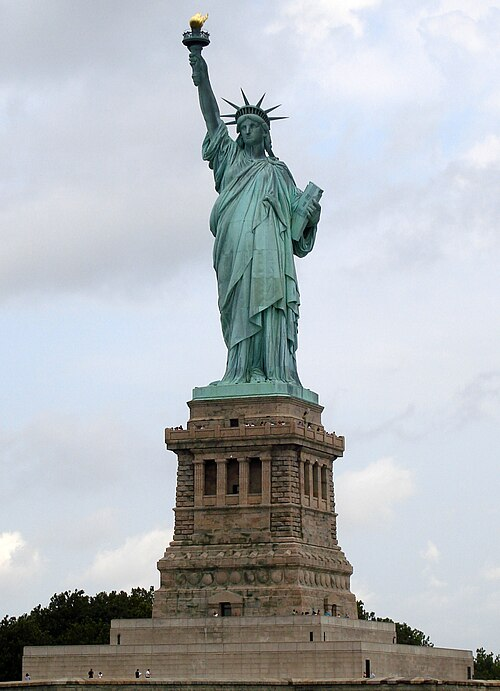
\includegraphics[width=0.32\linewidth]{images/book3/liberty.jpg}

{\small تمثال من النحاس عمره أكثر من قرن: صار جلده من صفائح النحاس الرقيقة
أخضر، تغطيه طبقة زنجار من أملاح النحاس القاعدية تحمي
الفلز تحتها. (صورة: إلكوبولا، ملكية عامة، ويكيميديا كومنز.)}
\end{omfigure}

\section{الحماية}

يُكافح التآكل بفصل الفلز عن الماء والأكسجين (الطلاء،
واللدائن، والمينا، أو طبقة من فلز آخر)، أو بتغيير الوسط
(نزع الأكسجين، وإضافة مثبطات تمتز على الفلز)، أو بإزاحة
جهد الفلز إلى منطقة مناعته.

\begin{definition}[الحماية المهبطية]\label{def:b2:corrosion:protection}
\emph{الحماية المهبطية}\index{حماية مهبطية} تخفض جهد
منشأة فلزية حتى تتوقف أكسدتها، بجعلها مهبط خلية.
ويمكن تكوين الخلية بواسطة \emph{مصعد مضحًّى}\index{مصعد مضحًّى}،
وهو فلز أقل نبلًا (الزنك، والمغنيسيوم، وسبائك الألومنيوم) موصول
بالمنشأة ويُستهلك مكانها، أو تشغيلها بمولّد، في
\emph{الحماية بالتيار المفروض}\index{حماية بالتيار المفروض}، ويكون
المصعد عندئذ قطبًا خاملًا مدفونًا بالقرب.
\end{definition}

\begin{proposition}[عمر مصعد مضحًّى]\label{prop:b2:corrosion:anode-life}
\omterm{def:b2:corrosion:protection}{المصعد المضحًّى} ذو الكتلة $m$ والكتلة المولية $M$، المتأكسد مع $n$ إلكترونًا
وبمردود $\eta$ (كسر الفلز الذي ينتج تيارًا
نافعًا، ويتآكل الباقي من تلقاء نفسه)، يعطي تيارًا $I$ مدة
\[
  t = \frac{\eta\,m\,nF}{M I} .
\]
\end{proposition}

\begin{proof}
الشحنة النافعة $\eta\,(m/M)\,nF$؛ نقسم على التيار.
\end{proof}

\begin{omfigure}
\begin{tikzpicture}[font=\small, >={Stealth}]
  \fill[brown!20] (-4.2,-2.4) rectangle (4.2,0);
  \draw[thick] (-4.2,0) -- (4.2,0);
  \node[font=\scriptsize, anchor=south west] at (-4.2,0) {سطح الأرض};
  \fill[black!40] (-3.5,-1.6) rectangle (3.5,-1.2);
  \node[font=\scriptsize, white] at (0,-1.4) {\shortstack{\foreignlanguage{arabic}{أنبوب فولاذي (مهبط)}}};
  % sacrificial anode
  \fill[black!65] (-3.2,-2.3) rectangle (-2.2,-1.95);
  \node[font=\scriptsize, anchor=north] at (-2.7,-2.3) {\foreignlanguage{arabic}{مصعد \babelsublr{Mg}}};
  \draw[thick] (-2.7,-1.95) -- (-2.7,-1.6);
  \draw[->, omProp, thick] (-2.2,-2.12) -- (-1.4,-1.7);
  \node[font=\scriptsize, omProp, anchor=west] at (-1.9,-2.2) {التيار في التربة};
  % impressed current
  \draw[thick, rounded corners] (1.8,0.4) rectangle (3.2,1.2);
  \node[font=\scriptsize] at (2.5,0.8) {مقوِّم};
  \fill[black!65] (3.4,-2.3) rectangle (3.9,-1.8);
  \node[font=\scriptsize, anchor=north] at (3.65,-2.3) {مصعد خامل};
  \draw[thick] (3.2,0.8) -- (3.65,0.8) -- (3.65,-1.8);
  \draw[thick] (1.8,0.8) -- (1.2,0.8) -- (1.2,-1.2);
  \node[font=\scriptsize, anchor=south] at (3.65,0.85) {$+$};
  \node[font=\scriptsize, anchor=south] at (1.2,0.85) {$-$};
  \node[font=\scriptsize, align=center] at (-2.7,0.8) {مصعد مضحًّى};
  \node[font=\scriptsize, align=center] at (2.5,1.55) {تيار مفروض};
\end{tikzpicture}

{\small \omterm{def:b2:corrosion:protection}{الحماية المهبطية} لأنبوب مدفون، رسم تخطيطي. يسارًا: مصعد من المغنيسيوم،
موصول بالأنبوب، يتآكل مكانه. يمينًا: مقوِّم يدفع
تيارًا من مصعد خامل عبر التربة إلى الأنبوب.}
\end{omfigure}

\begin{omfigure}
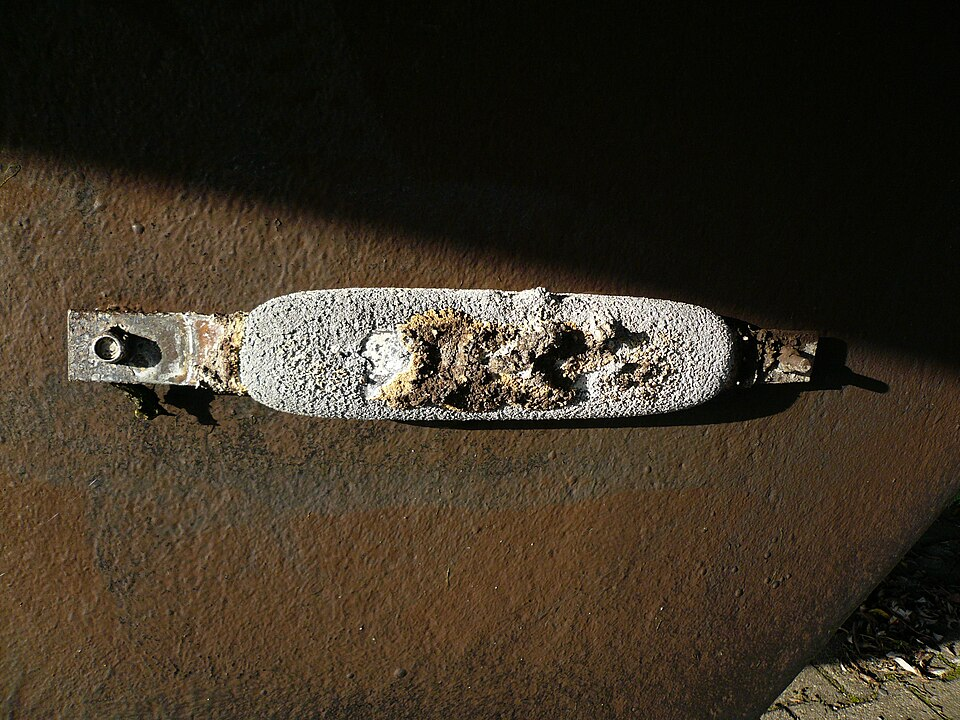
\includegraphics[width=0.5\linewidth]{images/book3/sacrificial-anode.jpg}

{\small \omterm{def:b2:corrosion:protection}{مصعد مضحًّى} من الزنك مثبَّت بالبراغي على هيكل فولاذي لقارب، بعد
موسم في الماء: الزنك متآكل، والفولاذ حوله سليم.
(صورة: تسفيرغلشترن، CC~BY-SA~3.0، ويكيميديا كومنز.)}
\end{omfigure}

\begin{omfigure}
\begin{tikzpicture}[font=\small, >={Stealth}, scale=1.35]
  \begin{scope}
    \fill[black!25] (0,0) rectangle (4,0.6);
    \fill[gray!55] (0,0.6) rectangle (1.7,0.8); \fill[gray!55] (2.3,0.6) rectangle (4,0.8);
    \fill[omDef!15] (0.8,0.8) .. controls (1.3,1.3) and (2.7,1.3) .. (3.2,0.8) -- (2.3,0.8) -- (2.3,0.6) -- (1.7,0.6) -- (1.7,0.8) -- cycle;
    \node[font=\scriptsize] at (2,-0.3) {\shortstack{\foreignlanguage{arabic}{فولاذ مجلفن (طبقة زنك)}}};
    \node[font=\scriptsize, align=center] at (2,1.6) {\foreignlanguage{arabic}{الزنك يتآكل،}\\ الفولاذ محمي};
    \draw[->, omThm] (1.4,0.85) -- (1.8,0.65);
  \end{scope}
  \begin{scope}[xshift=5.5cm]
    \fill[black!25] (0,0) rectangle (4,0.6);
    \fill[gray!25] (0,0.6) rectangle (1.7,0.8); \fill[gray!25] (2.3,0.6) rectangle (4,0.8);
    \fill[omDef!15] (0.8,0.8) .. controls (1.3,1.3) and (2.7,1.3) .. (3.2,0.8) -- (2.3,0.8) -- (2.3,0.6) -- (1.7,0.6) -- (1.7,0.8) -- cycle;
    \fill[omProp] (1.75,0.6) rectangle (2.25,0.45);
    \node[font=\scriptsize] at (2,-0.3) {\shortstack{\foreignlanguage{arabic}{فولاذ مقصدر (طبقة قصدير)}}};
    \node[font=\scriptsize, align=center] at (2,1.6) {\shortstack{\foreignlanguage{arabic}{الفولاذ يتآكل في الخدش،}\\\foreignlanguage{arabic}{بسرعة (مصعد صغير)}}};
  \end{scope}
\end{tikzpicture}

{\small خدش عبر طلاء فلزي، رسم تخطيطي. الزنك، الأقل نبلًا من
الحديد، يصير المصعد ويحمي الفولاذ المكشوف، أيًّا كان حجم
الخدش. أما القصدير، الأنبل من الحديد، فيصير مهبطًا كبيرًا حول مصعد
فولاذي صغير، يتآكل أسرع مما كان سيتآكل الفولاذ العاري.}
\end{omfigure}

\begin{method}[اختيار حماية]\label{met:b2:corrosion:choose-protection}
\begin{enumerate}
  \item تجنّب الأزواج الغلفانية: اعزل الفلزات المختلفة، أو اجعل الأقل
        نبلًا هو الأكبر.
  \item اطلِ: الطلاء العازل (الدهان، القصدير) لا يحمي إلا ما دام سليمًا؛ والطلاء
        المضحّي (الزنك) يحمي حتى حين يُخدش.
  \item لمنشأة في التربة أو في ماء البحر، أضف \omterm{def:b2:corrosion:protection}{الحماية المهبطية}:
        مصاعد مضحّاة للتيارات الصغيرة أو الماء الموصل،
        وتيارًا مفروضًا للمنشآت الطويلة أو التربة المقاومة.
  \item لا تبالغ في الحماية: فالجهد المنخفض جدًا يختزل الماء إلى هيدروجين عند
        المنشأة، وهو ما يرفع الطلاءات وقد يقصف أنواع الفولاذ
        العالية المقاومة.
\end{enumerate}
\end{method}

\section{تمارين}

\begin{exercise}[$\star$]\label{exo:b2:corrosion:1}
يتآكل الزنك تآكلًا منتظمًا تحت كثافة تيار قدرها \qty{2.0}{\micro A/cm^2}.
احسب ما يفقده من سمكه في السنة ($\rho = \qty{7.13}{g/cm^3}$).
\end{exercise}

\begin{exercise}[$\star$]\label{exo:b2:corrosion:2}
براغٍ من الفولاذ تثبّت صفائح نحاسية على سطح. أي الفلزين يتآكل؟ والسؤال نفسه
لمسامير من الزنك في صفائح فولاذية.
\end{exercise}

\begin{exercise}[$\star$]\label{exo:b2:corrosion:3}
تُشد صفيحتان فولاذيتان ببرغي وتُتركان في ماء البحر. أين يتركز
التآكل، ولماذا؟
\end{exercise}

\begin{exercise}[$\star$]\label{exo:b2:corrosion:4}
يُخدش دلو مجلفن وعلبة مقصدرة حتى الفولاذ. أيهما
يصدأ عند الخدش؟
\end{exercise}

\begin{exercise}[$\star\star$]\label{exo:b2:corrosion:5}
على مخطط إيفانز للحديد في الماء المهوّى، فسّر ما يحدث \omterm{def:b2:corrosion:uniform}{لجهد التآكل}
وتياره حين يُحرَّك الماء، ثم حين
يُنزع منه الأكسجين.
\end{exercise}

\begin{exercise}[$\star\star$]\label{exo:b2:corrosion:6}
يحمي مصعد من الزنك كتلته \qty{5.0}{kg} هيكل قارب بتيار قدره
\qty{0.10}{A}، بمردود قدره 90~\% (معطيات تمرين). كم
يدوم؟
\end{exercise}

\begin{exercise}[$\star\star$]\label{exo:b2:corrosion:7}
احسب الشحنة، بالأمبير ساعي لكل كيلوغرام، التي تعطيها مصاعد الزنك والمغنيسيوم
والألومنيوم بمردود 100~\%، والجهود المعيارية لمزدوجاتها
من $\Delta_f G^\circ$ (\ce{Zn^2+} $-147.06$، \ce{Mg^2+} $-454.8$،
\ce{Al^3+} $-485$ \unit{kJ/mol}). لماذا يُفضَّل المغنيسيوم في الترب الجافة؟
\end{exercise}

\begin{exercise}[$\star\star$]\label{exo:b2:corrosion:8}
يحتاج أنبوب مدفون إلى \qty{2.0}{A} من تيار الحماية. ولفراش المصعد
الخامل مقاومة قدرها \qty{4.0}{\ohm} بالنسبة إلى التربة وتحتاج الخلية
\qty{1.5}{V} إضافية (معطيات تمرين). احسب جهد المقوِّم 
والطاقة الكهربائية في السنة.
\end{exercise}

\begin{exercise}[$\star\star$]\label{exo:b2:corrosion:9}
ركيزة فولاذية قائمة في البحر. فسّر لماذا يكون تآكلها أشد تحت
خط الماء بقليل، لا عند خط الماء نفسه.
\end{exercise}

\begin{exercise}[$\star\star\star$]\label{exo:b2:corrosion:10}
فسّر، بمنحنى \omterm{def:b2:corrosion:passivation}{التخميل}، لماذا يقاوم الفولاذ المقاوم للصدأ الماء المهوّى لكنه
قد يتنقر في ماء البحر، ولماذا تنمو النقرة، بعد أن تبدأ، عمقًا لا
اتساعًا.
\end{exercise}

\begin{exercise}[$\star\star\star$]\label{exo:b2:corrosion:11}
تُثبَّت قطعة وصل نحاسية على أنبوب فولاذي ينقل ماءً مهوّى. كثافة
\omterm{def:b2:current-potential-curves:limiting-current}{التيار الحدي} للأكسجين \qty{5}{\micro A/cm^2} على كل سطح مبلل؛ ويقدّم
النحاس \qty{20}{cm^2} والفولاذ القريب من الوصلة \qty{2}{cm^2}
(معطيات تمرين). قدّر تيار تآكل الفولاذ وما يفقده من
سمكه في السنة قرب الوصلة.
\end{exercise}

\begin{exercise}[$\star\star\star$]\label{exo:b2:corrosion:12}
مستعملًا مخطط الجهد--pH للحديد ومنحنيات الماء، فسّر لماذا ينبغي إبقاء
جهد منشأة فولاذية محمية تحت نحو
\qty{-0.6}{V} لكن لا بعيدًا تحت \qty{-1}{V} في الماء المتعادل.
\end{exercise}

\section{مسألة: حماية خط أنابيب}

\begin{problem}[{مسألة نهاية الأسبوع --- تآكل أنبوب فولاذي عارٍ في تربة
رطبة، واختيار فلز مضحًّى، والمغنيسيوم اللازم لعشرين سنة،
وبديل التيار المفروض}]
\label{pb:b2:corrosion:1}
خط أنابيب فولاذي طوله \qty{10.0}{km} وقطره \qty{0.30}{m} مدفون في
تربة رطبة. المعطيات: الحديد $M = \qty{55.845}{g/mol}$، $\rho = \qty{7.87}{g/cm^3}$؛
المغنيسيوم $M = \qty{24.305}{g/mol}$؛ $\Delta_f G^\circ$ (\unit{kJ/mol}): \ce{Fe^2+}
$-78.90$، \ce{Zn^2+} $-147.06$، \ce{Mg^2+} $-454.8$، \ce{Al^3+} $-485$. ومعطيات
التمرين: كثافة تيار تآكل الفولاذ العاري في هذه التربة \qty{10}{\micro A/cm^2}؛ وكثافة التيار
التصميمية لحماية الفولاذ العاري \qty{20}{mA/m^2}؛ ويترك الطلاء 1.0~\% من السطح عاريًا؛
ومصاعد المغنيسيوم كتلة كل منها \qty{15}{kg}، بمردود 50~\%؛ ومقاومة فراش المصعد للتيار
المفروض \qty{5.0}{\ohm}.
% ledger: aw:Fe, rho:Fe, aw:Mg, dfg:Fe2+_ao, dfg:Zn2+_ao, dfg:Mg2+_ao, dfg:Al3+_ao, const:F

\medskip
\noindent\textbf{الجزء الأول --- الأنبوب العاري.}
\begin{enumerate}
  \item اكتب التفاعلين المصعدي والمهبطي على الأنبوب.
  \item لماذا يحدد إمدادُ الأكسجين تيارَ التآكل؟
  \item احسب كتلة الحديد المفقودة لكل متر مربع وفي السنة.
  \item احسب ما يُفقد من سمك الجدار في السنة.
  \item كم من الوقت يحتاج الأنبوب العاري ليفقد نصف جدار سمكه \qty{8}{mm}؟
  \item لماذا يتلف الأنبوب الحقيقي أبكر من ذلك، عند بضع نقاط؟
\end{enumerate}

\medskip
\noindent\textbf{الجزء الثاني --- فلز المصعد.}
\begin{enumerate}[resume]
  \item احسب الجهود المعيارية لمزدوجات الحديد والزنك والمغنيسيوم
        والألومنيوم.
  \item أي الفلزات تستطيع حماية الحديد مصاعدَ مضحّاة؟
  \item لماذا يقل استعمال الألومنيوم في الترب؟
  \item لماذا يُفضَّل المغنيسيوم على الزنك في تربة عالية المقاومية؟
  \item احسب كتلة المغنيسيوم المستهلكة لكل أمبير وفي السنة.
\end{enumerate}

\medskip
\noindent\textbf{الجزء الثالث --- التصميم.}
\begin{enumerate}[resume]
  \item احسب السطح الخارجي للأنبوب.
  \item احسب السطح العاري الذي يتركه الطلاء.
  \item احسب تيار الحماية.
  \item احسب الشحنة اللازمة لعشرين سنة.
  \item احسب كتلة المغنيسيوم اللازمة.
  \item كم مصعدًا يلزم؟
  \item لماذا تُوزَّع على طول الأنبوب بدل دفنها في
        نقطة واحدة؟
\end{enumerate}

\medskip
\noindent\textbf{الجزء الرابع --- التيار المفروض.}
\begin{enumerate}[resume]
  \item صِف بديل التيار المفروض.
  \item قدّر جهد المقوِّم من مقاومة فراش المصعد،
        مضيفًا \qty{1.5}{V} للأقطاب.
  \item احسب الطاقة الكهربائية المستعملة في السنة.
  \item ماذا يسوء إذا بولغ في حماية الأنبوب؟
  \item تحت أي جهد يكون الحديد منيعًا في الماء المتعادل، مع أخذ
        تركيز للحديد(II) قدره \qty{1e-6}{mol/L}؟
  \item اذكر كتلة مصاعد المغنيسيوم اللازمة لعشرين سنة.
\end{enumerate}
\end{problem}
